\documentclass[11pt]{standalone}

\usepackage{amssymb} 
\usepackage{amsmath} 

\usepackage[no-math]{fontspec}
\usepackage{unicode-math}
\setmainfont{Lato}
\setmathfont{Stix Two Math}

\usepackage{tikz}
\usetikzlibrary{arrows.meta}
\usepackage{pgfplots}
\pgfplotsset{compat=newest}
\usetikzlibrary{backgrounds}

\usepackage{xcolor}
\definecolor{accent1}{RGB}{0,90,148}
\definecolor{accent2}{RGB}{204,222,233}
\definecolor{alert}{RGB}{230,0,0}
\definecolor{bg}{RGB}{243,244,244}
\definecolor{fg}{RGB}{72,73,73}


\makeatletter
\tikzset{fixed ratio/.code={\def\tikz@pft##1:##2;{\edef\pgfutil@tempx{##1}\edef\pgfutil@tempy{##2}}%
    \expandafter\tikz@pft#1;%
    \tikzset{execute at end picture={%
    \ifcsname sa@border@right\endcsname
     \pgfmathsetmacro\pgfutil@tempa{((\pgf@picmaxx+\sa@border@right-\pgf@picminx+\sa@border@left)/%
     (\pgf@picmaxy+\sa@border@top-\pgf@picminy+\sa@border@bottom)}%
    \else
     \pgfmathsetmacro\pgfutil@tempa{((\pgf@picmaxx-\pgf@picminx)/(\pgf@picmaxy-\pgf@picminy)}%
    \fi
    \pgfmathsetmacro\pgfutil@tempb{(\pgfutil@tempx/\pgfutil@tempy)}%
    \ifdim\pgfutil@tempa pt=\pgfutil@tempb pt\relax
    \else
     \ifdim\pgfutil@tempb pt>\pgfutil@tempa pt\relax
      % target ratio greater than actual
      \pgfmathsetmacro\pgfutil@tempc{-(\pgf@picmaxx-\pgf@picminx)%
      +\pgfutil@tempb*(\pgf@picmaxy-\pgf@picminy)}%
      \path ([xshift=-0.5*\pgfutil@tempc]current bounding box.west)
       ([xshift=0.5*\pgfutil@tempc]current bounding box.east);
     \else
      % target ratio smaller than actual
      \pgfmathsetmacro\pgfutil@tempc{-(\pgf@picmaxy-\pgf@picminy)%
      +(\pgf@picmaxx-\pgf@picminx)/\pgfutil@tempb}%
      \path ([yshift=-0.5*\pgfutil@tempc]current bounding box.south)
       ([yshift=0.5*\pgfutil@tempc]current bounding box.north);
     \fi
    \fi
    }%  
    }}
}
\makeatother



\usetikzlibrary{angles, quotes}
\usetikzlibrary{decorations.pathreplacing, calligraphy}
\usepackage{scalefnt}

\begin{document}
{\scalefont{0.5}
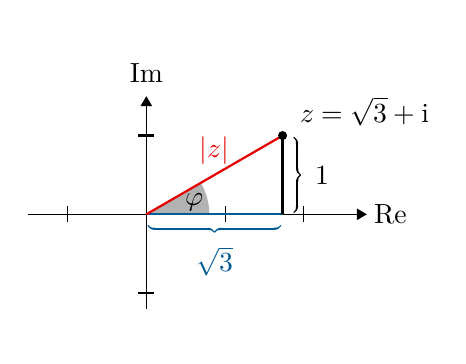
\begin{tikzpicture}[fixed ratio=4:3]
	% x-axis	
	\draw [-{Triangle}] (-1.5,0) -- (2.8,0);
	\draw (3.1,0) node {Re};
	% negative part of x-axis
	\foreach \x in {-1,...,-1} {
        \draw (\x,-.1) -- (\x,0.1);
        % \draw (\x,-0.4) node {$\x$};  
    }
    % positive part of x-axis
    \foreach \x in {1,...,2} {
        \draw (\x,-.1) -- (\x,0.1);
        % \draw (\x,-0.4) node {$\x$};   
    }
    % y-axis
   	\draw [-{Triangle}] (0,-1.2) -- (0,1.5);
	% negative part of y-axis
    \foreach \x in {-1,...,-1} {
        \draw [thick] (-.1,\x) -- (0.1,\x);
        % \draw (-0.4,\x) node {$\x$};    
    }
    % positive part of y-axis
    \foreach \x in {1,...,1} {
        \draw [thick] (-.1,\x) -- (0.1,\x);
        % \draw (-0.4,\x) node {$\x$};    
    }
    \draw (0,1.8) node {Im};

    % points
  	\draw[] (1.73,0) coordinate (A) -- (0,0) coordinate (B) -- (1.73,1) coordinate (C)
		pic [fill=black!30, angle radius=0.8cm, "$\varphi$" shift={(1.5mm,0.25mm)}] {angle = A--B--C};
	\draw[pen colour=accent1, decorate, decoration = {calligraphic brace, mirror, raise=4pt}, thick] (0.02,0) --  (1.71,0) node[pos=0.5,below=8pt,accent1]{$\sqrt{3}$}; 
	\draw[pen colour=black, decorate, decoration = {calligraphic brace, mirror, raise=4pt}, thick] (1.73,0.02) --  (1.73,0.98) node[pos=0.5,right=8pt]{$1$}; 		
    \draw [thick, color=accent1] (0,0) -- (1.73,0);
    \draw [thick, color=black] (1.73,0) -- (1.73,1);
    \draw [thick, color=alert] (0,0) -- node[above] {$|z|$} (1.73,1);
    \draw [fill] (1.73,1) node [anchor=south west] {$\; z = \sqrt{3} + \mathrm{i}$} circle (0.05);
\end{tikzpicture}
}
\end{document}